In a Bayesian treatment of  hyper-parameter learning for \ac{GP}s,
we can write the probability of the hyper-parameters of a GP as
defined above, given covariance function $\mathbf{K}$ as:
\begin{equation}
\label{eq:hyperProbability}
P(\bm{\theta} \mid \mathbf{D,K}) = \frac{P(\mathbf{D} \mid \bm{\theta}, \mathbf{K})P(\bm{\theta} \mid  \mathbf{K})}{P(\mathbf{D} \mid \mathbf{K})}.
\end{equation}
Let the $\mathbf{K}$ be the sum of a smoothing and a white noise (WN) kernel. For this case, Neal~\citeyearpar{neal1997monte} suggested the problem of outliers in data as a use-case for a hierarchical Bayesian treatment of Gaussian processes\footnote{In Neal's work \citeyearpar{neal1997monte} the sum of an SE plus a constant kernel is used. We keep the WN kernel for illustrative purposes.}. The work suggests a hierarchical system of hyper-parameterization. Here, we draw hyper-parameters from a $\Gamma$ distributions:
\begin{equation}
\label{eq:hyper-ell}
\ell^{(t)} \sim \Gamma(\alpha_1,\beta_1),\;\sigma^{(t)} \sim \Gamma(\alpha_2,\beta_2)
\end{equation} 
and in turn sample the $\alpha$ and $\beta$ from $\Gamma$ distributions as well:
\begin{equation}
\label{eq:hyper-alpha}
\alpha_1^{(t)} \sim \Gamma(\alpha^1_{\alpha},\beta^1_{ \alpha } ),\; \alpha_2^{(t)} \sim \Gamma(\alpha^2_{\alpha},\beta^2_{\alpha}),\cdots
\end{equation}
% the input below will be empty, if we're in the paper. For my thesis, it will contain a causal network of the hyper-parameters.
One can represent this kind of model using \gpmem\ (Fig. \ref{fig:neal_tutorial}).
Neal provides a custom inference algorithm setting and evaluates it using the following synthetic data problem. Let $f$ be the underlying function that generates the data:
\begin{equation}
f(x) =  0.3 + 0.4 x + 0.5 \sin(2.7x) + \frac{1.1}{(1+ x^2)} + \eta \;\;\; with\;\;\eta \sim \mathcal{N}(0,\sigma)
\end{equation}
We synthetically generate outliers by setting $\sigma = 0.1$ in $95\%$ of the cases and to $\sigma = 1$ in the remaining cases. \gpmem\  can capture the true underlying function within only 100 MH steps on the hyper-parameters to get a good approximation for their posterior. Note that Neal devises an additional noise model and performs a large number of Hybrid-Monte Carlo and Gibbs steps.  
\begin{comment}
 
\begin{figure}
\begin{subfigure}[b]{0.49\textwidth}\centering
\begin{tabular}{ll}
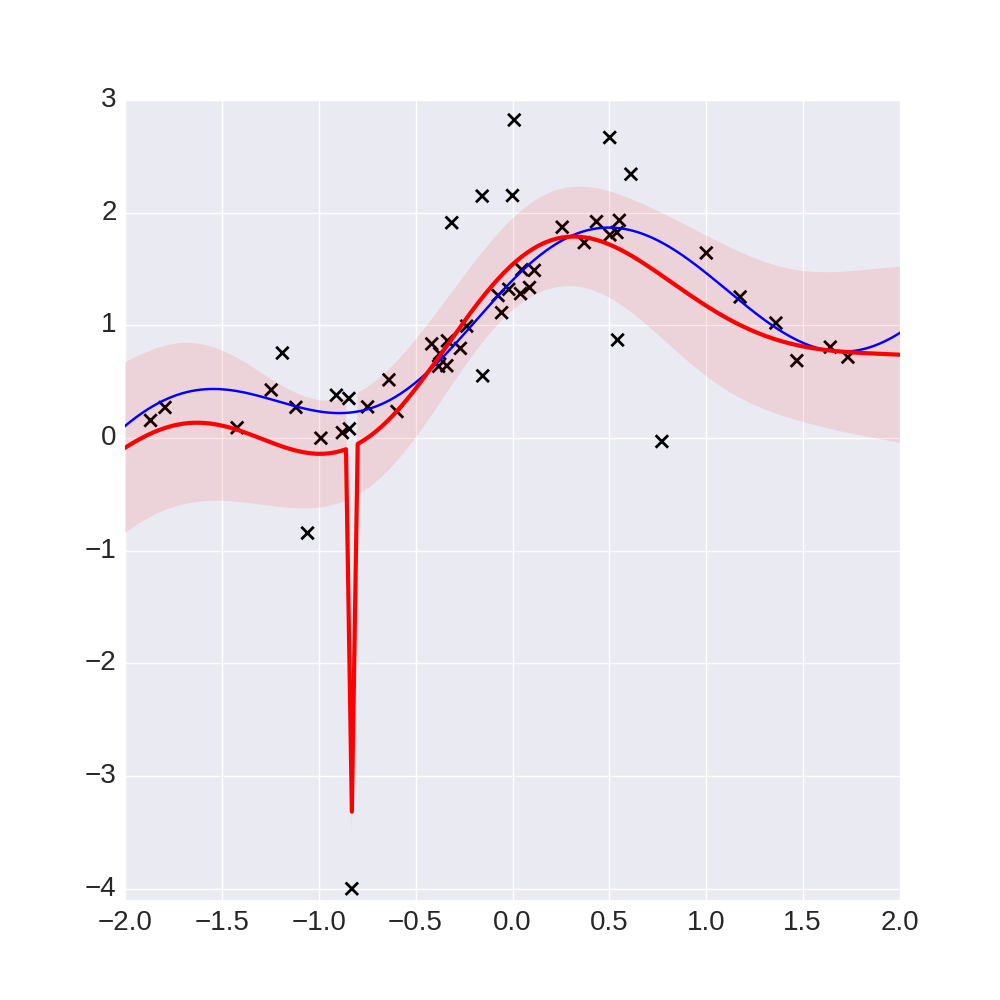
\includegraphics[height=4.5cm]{figs/neal_deterministic.png} &  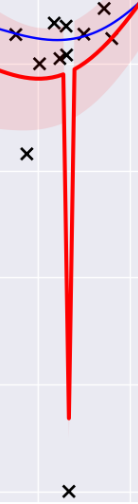
\includegraphics[height=4.5cm]{figs/outlier.png}
\end{tabular}
          \caption{}
          \label{fig:deterministic}
\end{subfigure}          
\begin{subfigure}[b]{0.49\textwidth}\centering
\centering
\begin{tabular}{ll}
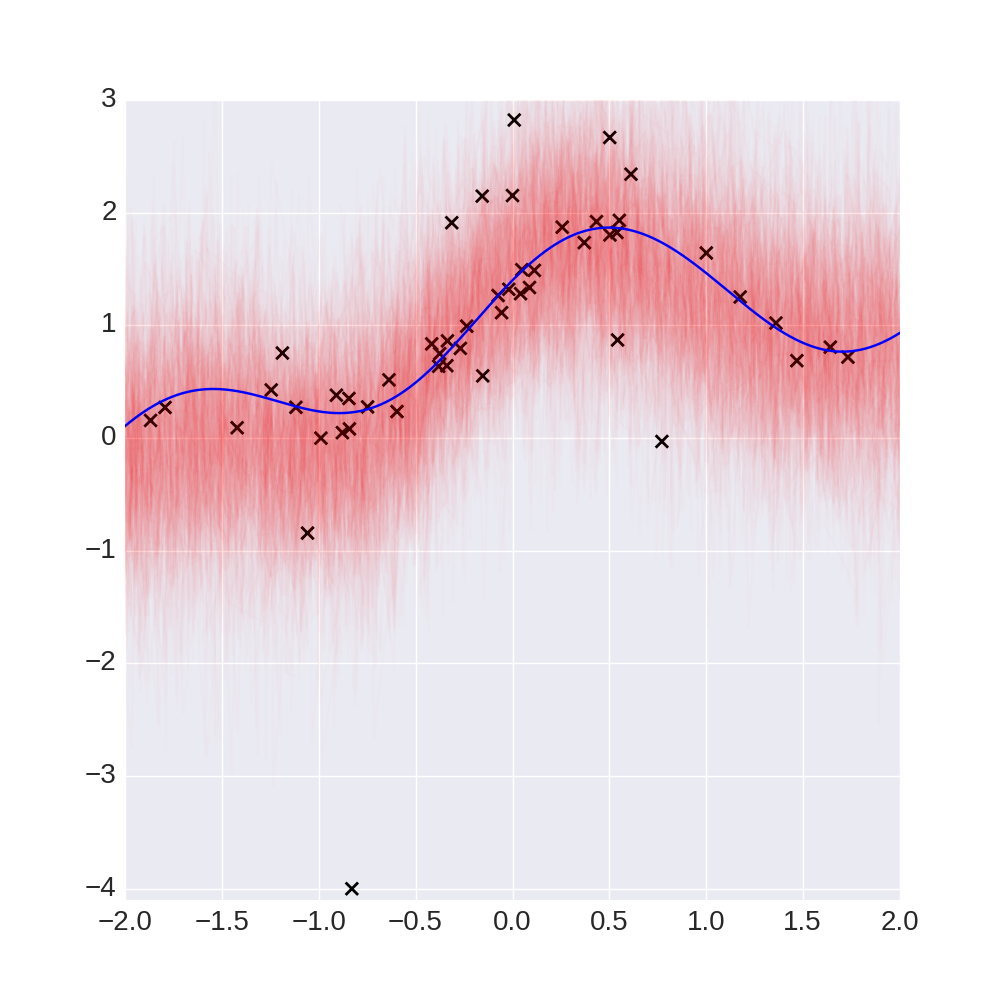
\includegraphics[height=4.5cm]{figs/neal_Bayesian.png} &  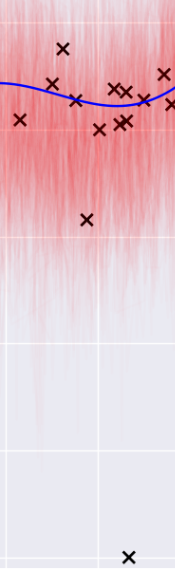
\includegraphics[height=4.5cm]{figs/outlier_Bayesian.png}
\end{tabular}
          \caption{}
          \label{fig:Bayesian}
\end{subfigure}
        		\put(-130,55){\color{green}\thicklines \vector(1,0){80}}
        		\put(-326,55){\color{green}\thicklines \vector(1,0){80}}
			\put(-47,21){\color{green} \thicklines \line(1,0){39}}
			\put(-47,148){\color{green} \thicklines \line(1,0){39}}
		        \put(-47,21){\color{green} \thicklines \line(0,1){127}}
		        \put(-8,21){\color{green} \thicklines \line(0,1){127}}
		        \put(-243,21){\color{green} \thicklines \line(0,1){127}}
		        \put(-206,21){\color{green} \thicklines \line(0,1){127}}
		        \put(-243,21){\color{green} \thicklines \line(1,0){37}}
			\put(-243,148){\color{green} \thicklines \line(1,0){37}}
\caption{(a) a shows deterministic inferece, that is optimization for an example of Neals synthetic function with an extreme outlier (green).}\label{fig:neal}
\end{figure}


\end{comment}



\begin{figure}
\renewcommand{\arraystretch}{0.1}% Tighter
\centering \footnotesize
\begin{tikzpicture}
\node[] (start) {};
\node[left=1cm of start] (sfsigma) {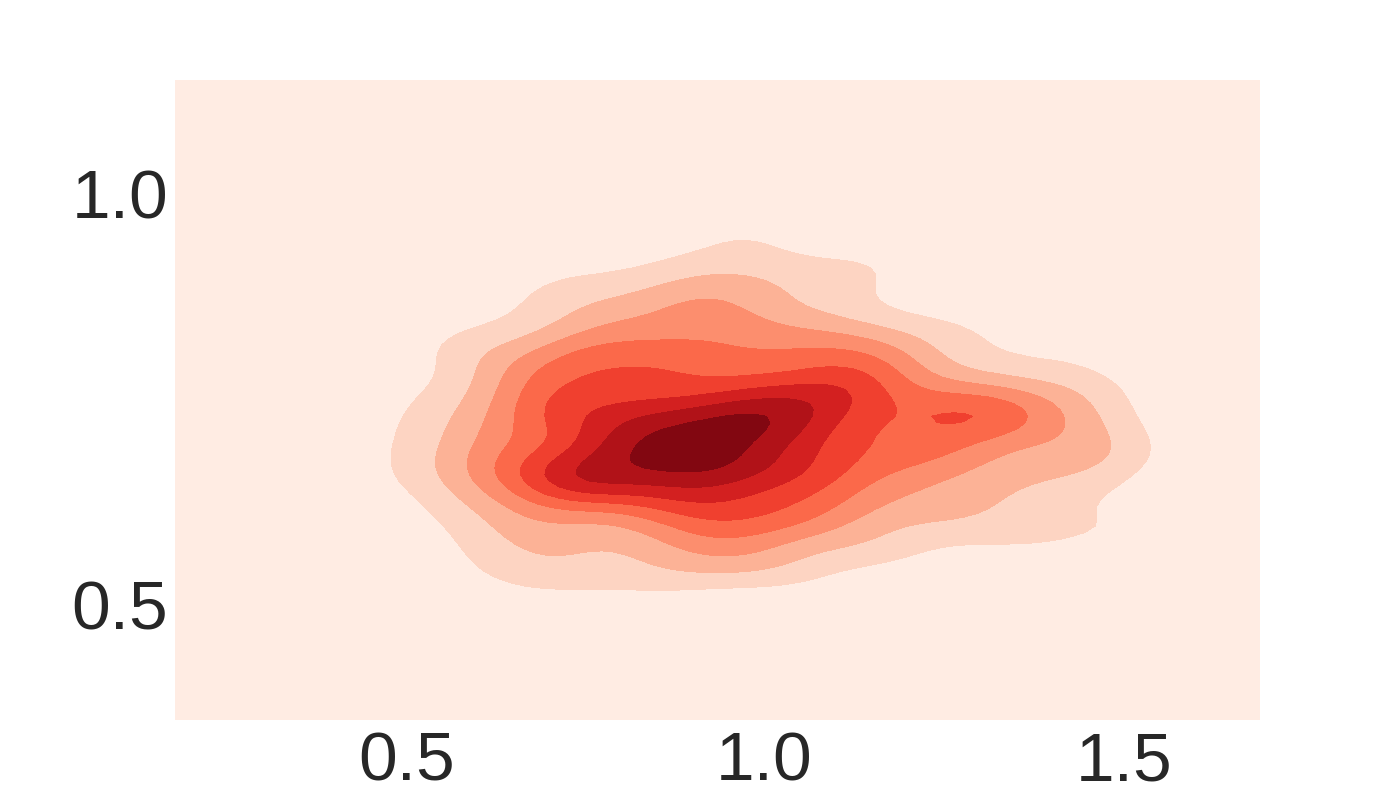
\includegraphics[height=2cm]{figs/hypers_sf_sigma.png}};
\node[right=1cm of start] (sfell) {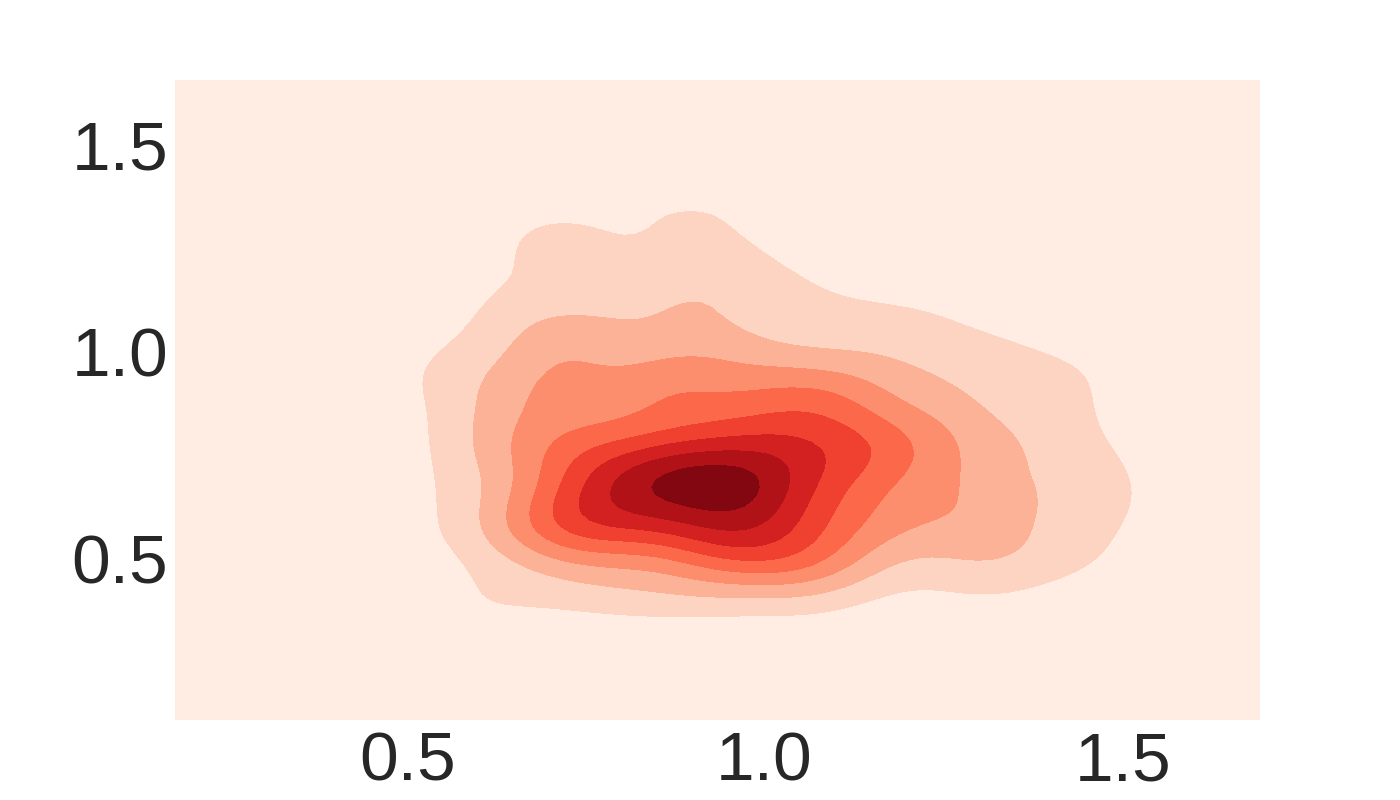
\includegraphics[height=2cm]{figs/hypers_sf_ell.png}};
\node[above=1cm of start] (hyper) {Hyper-Parameters for the Kernel:};
\node[left=0.cm of sfsigma] (ell) {$\ell$};
\node[below=0.cm of sfsigma] (sf1) {$sf$};
\node[left=0.cm of sfell] (sigma) {$\sigma$};
\node[below=0.cm of sfell] (sf2) {$sf$};
\end{tikzpicture}
\begin{tabular}{ll} \hline
\multicolumn{2}{}{}
  \begin{minipage}{4cm}
 \footnotesize\begin{lstlisting}
 // Data and look-up function
 define data = array(array(-1.87,0.13),..., array(1.67,0.81)) 
 assume f_look_up = proc(index) {lookup( data, index)}
\end{lstlisting}
\end{minipage}\\
\hline
\multicolumn{2}{}{}
  \begin{minipage}{4cm}
 \footnotesize\begin{lstlisting} 
 assume sf = tag(quote(hyper), 0, gamma(alpha_sf, beta_sf)))
 assume l = tag(quote(hyper), 1, gamma(alpha_l, beta_l)))
 assume sigma = tag(quote(hyper), 2, uniform_continuous(0, 2)) 
\end{lstlisting}
\end{minipage}
  \\
\hline
\footnotesize\begin{lstlisting}[ belowcaptionskip=0.1\baselineskip,mathescape,escapechar=\#]
// The covariance function
assume se = make_squaredexp(sf, l)
assume wn = make_whitenoise(sigma)
assume composite_covariance = add_funcs(se, wn)#\vspace{1mm}#
// Create a prober and emulator using gpmem
assume (f_compute, f_emu)
      = gpmem(f_look_up, composite_covariance)#\vspace{1mm}#
sample f_emu( array( -2, $\cdots$, 2)) 
\end{lstlisting}
 &  \raisebox{-0.5\height}{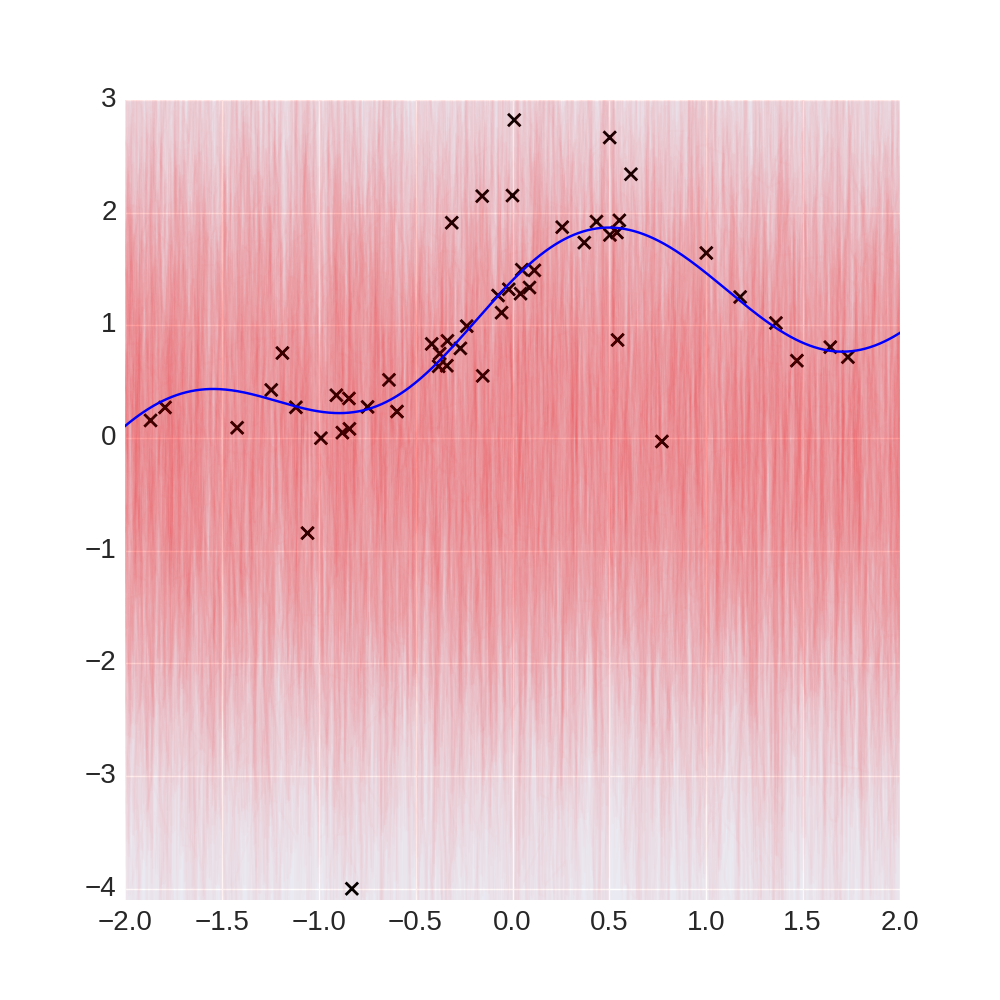
\includegraphics[height=3.4cm]{figs/neal_example_before_observation.png}}  \\ \hline
% line 3 

\footnotesize\begin{lstlisting}[aboveskip=-0.8 \baselineskip,mathescape,escapechar=\#]
// Observe all data points
for n ... N
    observe f_emu(first(lookup(data,n))) 
                = second(lookup(data,n))
// Or: probe all data points
for n ... N
    predict f_compute(first(lookup(data,n)))#\vspace{1mm}#
sample f_emu( array( -2, $\cdots$, 2)) 
\end{lstlisting}
 &  \raisebox{-0.5\height}{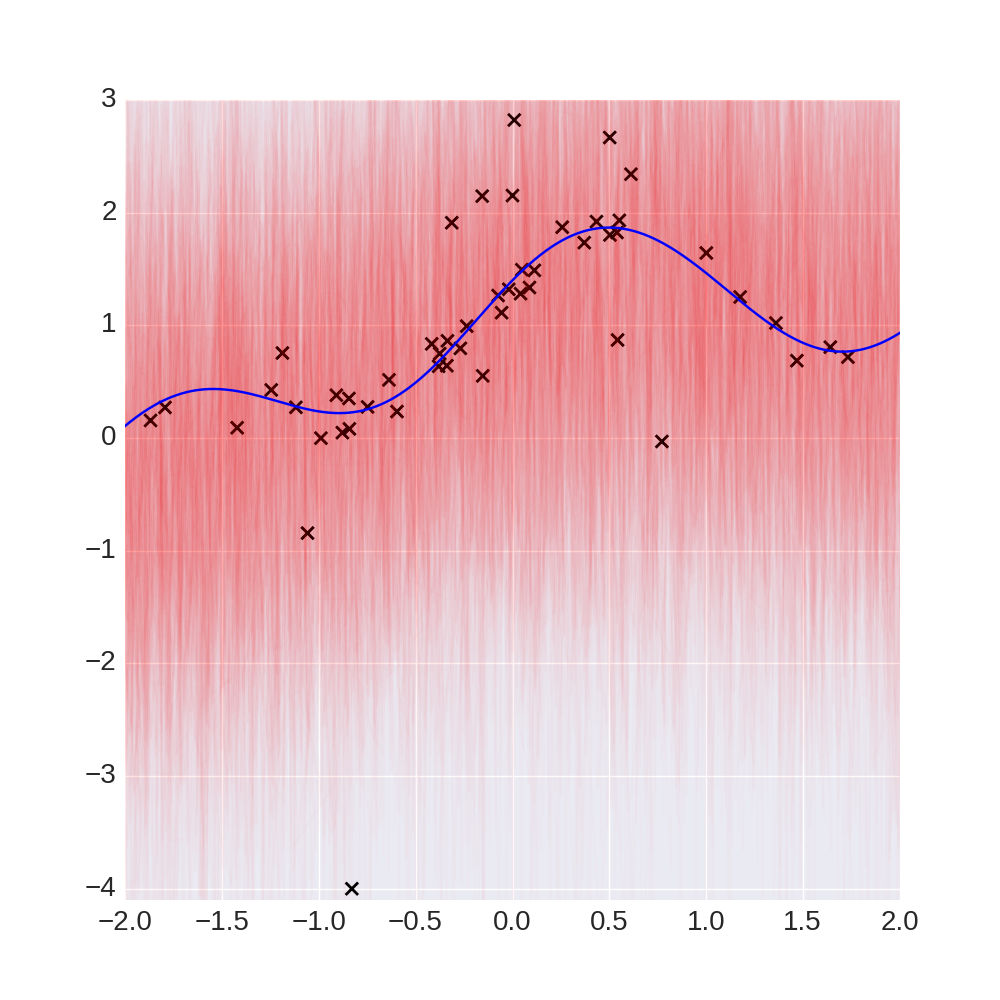
\includegraphics[height=3.4cm]{figs/neal_example_after_observation.png}}  \\ \hline
\footnotesize\begin{lstlisting}[mathescape,escapechar=\#]
// Metropolis-Hastings
infer repeat( 100, do(
                   mh( quote(hyperhyper), one, 2),
		   mh( quote(hyper),      one, 1)))#\vspace{1mm}#
sample f_emu( array( -2, $\cdots$, 2))   
\end{lstlisting}
 &   \raisebox{-0.5\height}{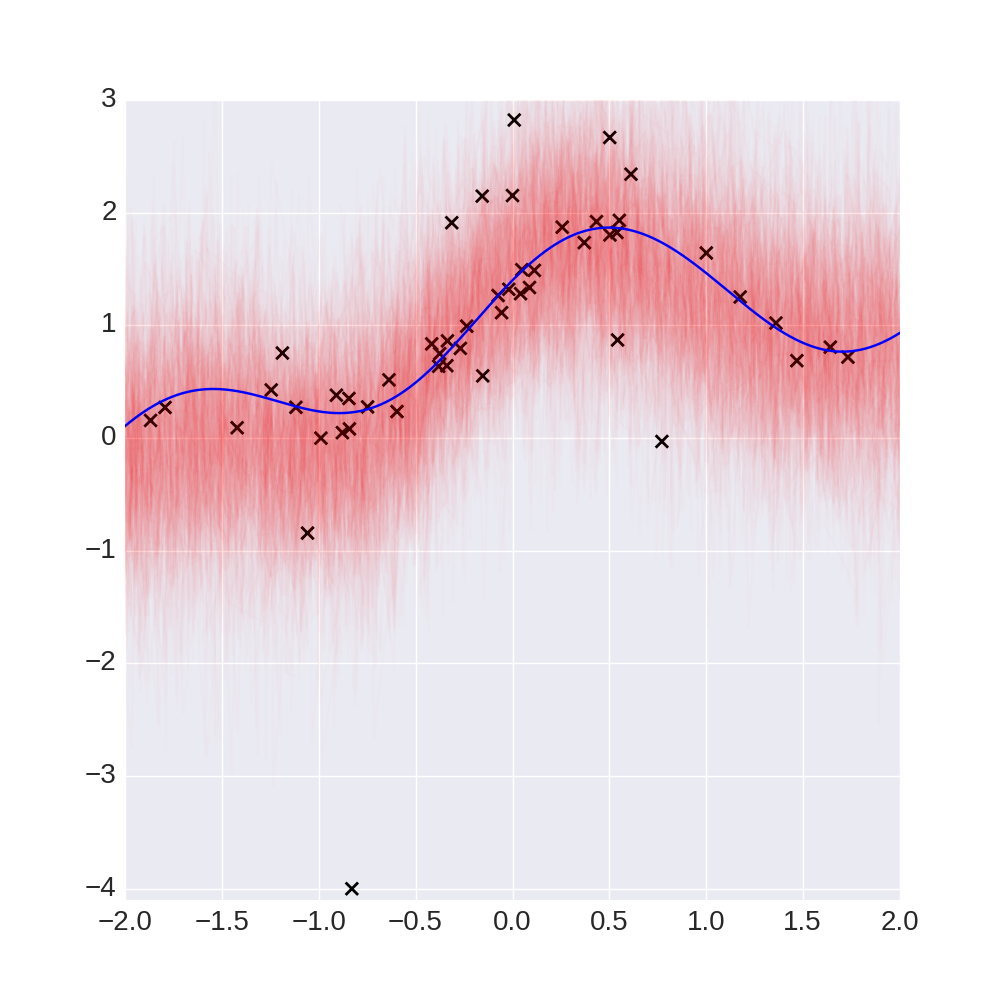
\includegraphics[height=3.4cm]{figs/neal_Bayesian.png}} \\ \hline
\footnotesize\begin{lstlisting}[mathescape,escapechar=\#]
// Optimization 
infer map( quote(hyper), all,0.01, 15)

sample f_emu( array( -2, $\cdots$, 2)) 
\end{lstlisting}
 &   \raisebox{-0.5\height}{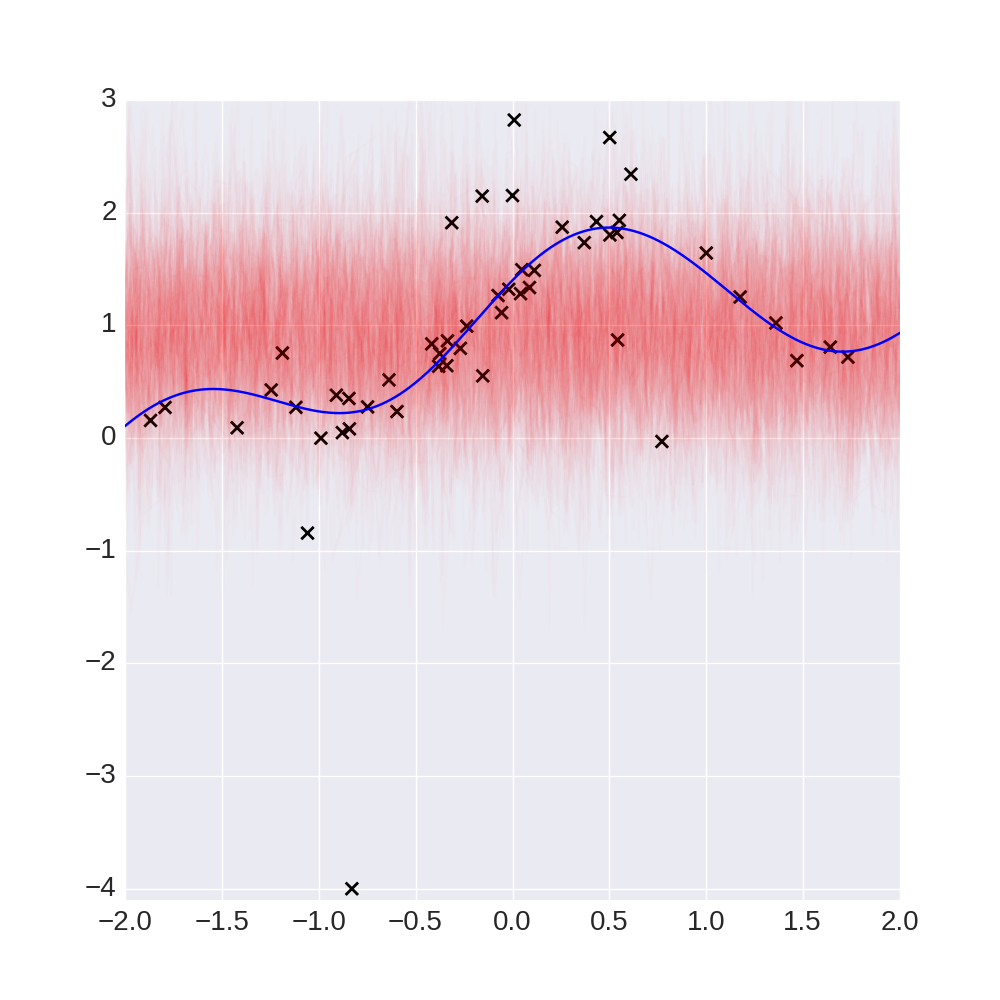
\includegraphics[height=3.4cm]{figs/neal_example_map_inference_alpha0p01_iter15.png}} \\ \hline
 
 \end{tabular}
\caption{Regression with outliers and hierarchical prior structure.}
\label{fig:neal_tutorial}
\end{figure}



